
%%%%%%%%%%%%%%%%%%%%%%%%%%%%%%%%%%%%%%%%%%%%%%%%%%%%%%%%%%%%%%%%%%%%%%%%%%%%%%%%%%%%%%%
%%%%%%%%%%%%%%%%%%%%%%%%%%%%%%%%%%%%%%%%%%%%%%%%%%%%%%%%%%%%%%%%%%%%%%%%%%%%%%%%%%%%%%%
% 
% This top part of the document is called the 'preamble'.  Modify it with caution!
%
% The real document starts below where it says 'The main document starts here'.

\documentclass[12pt]{article}

\usepackage{amssymb,amsmath,amsthm}
\usepackage[top=1in, bottom=1in, left=1.25in, right=1.25in]{geometry}
\usepackage{fancyhdr}
\usepackage{enumerate}
\usepackage{listings}
\usepackage{graphicx}
\usepackage{float}

\usepackage{mwe}
\usepackage{caption}
\usepackage{subcaption}
% Comment the following line to use TeX's default font of Computer Modern.
\usepackage{times,txfonts}



\makeatletter
\renewcommand*\env@matrix[1][*\c@MaxMatrixCols c]{%
  \hskip -\arraycolsep
  \let\@ifnextchar\new@ifnextchar
  \array{#1}}
\makeatother

\newtheoremstyle{homework}% name of the style to be used
  {18pt}% measure of space to leave above the theorem. E.g.: 3pt
  {12pt}% measure of space to leave below the theorem. E.g.: 3pt
  {}% name of font to use in the body of the theorem
  {}% measure of space to indent
  {\bfseries}% name of head font
  {:}% punctuation between head and body
  {2ex}% space after theorem head; " " = normal interword space
  {}% Manually specify head
\theoremstyle{homework} 

% Set up an Exercise environment and a Solution label.
\newtheorem*{exercisecore}{Exercise \@currentlabel}
\newenvironment{exercise}[1]
{\def\@currentlabel{#1}\exercisecore}
{\endexercisecore}

\newcommand{\localhead}[1]{\par\smallskip\noindent\textbf{#1}\nobreak\\}%
\newcommand\solution{\localhead{Solution:}}

%%%%%%%%%%%%%%%%%%%%%%%%%%%%%%%%%%%%%%%%%%%%%%%%%%%%%%%%%%%%%%%%%%%%%%%%
%
% Stuff for getting the name/document date/title across the header
\makeatletter
\RequirePackage{fancyhdr}
\pagestyle{fancy}
\fancyfoot[C]{\ifnum \value{page} > 1\relax\thepage\fi}
\fancyhead[L]{\ifx\@doclabel\@empty\else\@doclabel\fi}
\fancyhead[C]{\ifx\@docdate\@empty\else\@docdate\fi}
\fancyhead[R]{\ifx\@docauthor\@empty\else\@docauthor\fi}
\headheight 15pt

\def\doclabel#1{\gdef\@doclabel{#1}}
\doclabel{Use {\tt\textbackslash doclabel\{MY LABEL\}}.}
\def\docdate#1{\gdef\@docdate{#1}}
\docdate{Use {\tt\textbackslash docdate\{MY DATE\}}.}
\def\docauthor#1{\gdef\@docauthor{#1}}
\docauthor{Use {\tt\textbackslash docauthor\{MY NAME\}}.}
\makeatother

% Shortcuts for blackboard bold number sets (reals, integers, etc.)
\newcommand{\Reals}{\ensuremath{\mathbb R}}
\newcommand{\Nats}{\ensuremath{\mathbb N}}
\newcommand{\Ints}{\ensuremath{\mathbb Z}}
\newcommand{\Rats}{\ensuremath{\mathbb Q}}
\newcommand{\Cplx}{\ensuremath{\mathbb C}}
%% Some equivalents that some people may prefer.
\let\RR\Reals
\let\NN\Nats
\let\II\Ints
\let\CC\Cplx

%%%%%%%%%%%%%%%%%%%%%%%%%%%%%%%%%%%%%%%%%%%%%%%%%%%%%%%%%%%%%%%%%%%%%%%%%%%%%%%%%%%%%%%
%%%%%%%%%%%%%%%%%%%%%%%%%%%%%%%%%%%%%%%%%%%%%%%%%%%%%%%%%%%%%%%%%%%%%%%%%%%%%%%%%%%%%%%
% 
% The main document start here.

% The following commands set up the material that appears in the header.
\doclabel{STAT 401: Homework 8}
\docauthor{Stefano Fochesatto}
\docdate{\today}


%\begin{figure}[H]
%  \begin{center}
%  \caption{}
%  \includegraphics[\textwidth]{}
%  \end{center}
%\end{figure}

% \textbf{Code:}
% \begin{center}
% \lstinputlisting{}
% \end{center} 



\begin{document}

\begin{exercise}{1} Do problem 5.14. For part 1 use scatterplot() fumnction with the groups agrumet to get different 
  plotting symbols for males and females, as described in this week's lab. You will also need to turn BGsall\$sex ino a factor
  variable before you do part to 2 and 3. For part 2 testing the parallel regerssion model consists of testing the interaction
  term, since the interaction allows for non parallel slopers in HT9. For part 3, remember that the difference between males and females is 
  represented by a particular model coefficient hence you are asked to simple find a confidence interval ona  coeficient.\\

  Refer to the Berkely Guidence study decrived in Problem 3.3, Using data BGSall, consider the regression HT18 on HT9 and grouping factor Sex.\\

  \begin{enumerate}
    \item[5.14.1] Draw the scatterplot of HT18 versus HT9, using a different symbol for males and females. Comment on the 
    information in the graph about the apprpriate mean function for these data. \\
    \solution  Using scatterplot we get the following plot, 
    \begin{figure}[H]
      \begin{center}
      \caption{Boys vs Girls Predicted Height in Centimeters}
      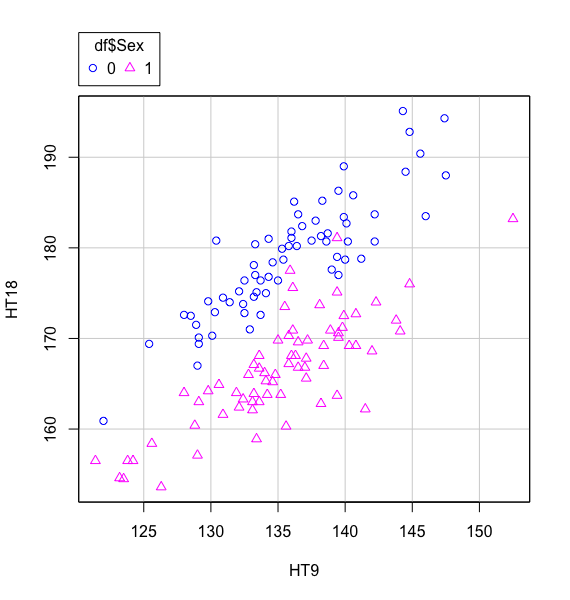
\includegraphics[width = .66\textwidth]{Rplot.png}
      \end{center}
     \end{figure}    
       \textbf{Code:}
       \begin{center}
       \lstinputlisting[basicstyle = \small]{r1.txt}
       \end{center} 
       As expected we can see that if we fitted the straight line mean function to the data, the boys average height would be greater than the girls. Looking 
       at the data I'd imagine that fitting an SLR to each data we would get very similar slope coefficients and a significant difference in intercepts. 
       \newpage


       \item[5.14.2] Obtain the appropriate test for a parallel regression model. \\
       \solution  To see if a parallel regression model is sufficient for this data we need to test the significance of the interaction term 
       of the general model. Using the Type-2 Partial F test(Anova) we get that the interaction term is significant on the $alpha = .05$ level.
       Looking at the data it seems that a parallel model would be sufficient but it doesn't hurt to include the interaction term. \\
       \textbf{Code:}
       \begin{center}
       \lstinputlisting[basicstyle = \small]{r2.txt}
       \end{center}
       \newpage



       \item[5.14.3] Assuming the parallel regression model is adequate, estimate a 95 percent 
       confidence interval for the difference between males and females. For the parallel repression model, 
       this is the difference in the intercepts of the two groups.  \\
       \solution As stated previosly the difference between males and females in the data is encoded in the 
       Sex coefficient of the parallel regression model. We can see this by setting all other predictors to zero and computing the 
       intercept for both males and females, as expected the difference is the coefficient of the Sex predictor. To compute the difference we simply need to find the confidence 
       interval for that regresison coefficient. \\
       \textbf{Code:}
       \begin{center}
       \lstinputlisting[basicstyle = \small]{r3.txt}
       \end{center}
  \end{enumerate} 
\end{exercise}
\newpage

\begin{exercise}{2} do Proble, 5.17. In part 1 all you need to do is get the scatterplot between salary and year, with 
  different plotting symbol for the levels of sex. In part 2, use a simple two-sample t-test. In part 3 use the parallel 
  regression model. Skip part 4.
   \begin{enumerate}
     \item[5.17.1] Get appropriate graphical summaries of the data and discuss the graphs.\\ 
     \solution Plotting salary as the response with year and sex as predictors we get the following, 
     \begin{figure}[H]
      \begin{center}
      \caption{Salaries vs Tenure for Both Male and Female Employees}
      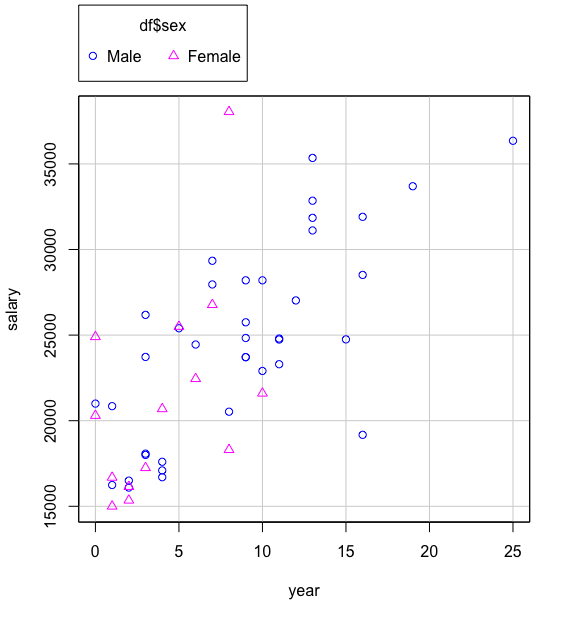
\includegraphics[width = .66\textwidth]{Rplot01.png}
      \end{center}
     \end{figure}    
       \textbf{Code:}
       \begin{center}
       \lstinputlisting[basicstyle = \small]{r4.txt}
       \end{center}  
       From the scatterplot we can see that generally there are fewer female employees. The female employees also have a significant 
       earnings ceiling, when compared to male earnings. A majority of female employees are below the 27,000 dollar earnings, while there seems to be a 
       a significant proportion of male employees which have higher earnings that that.\\
       \newpage

       \item[5.17.2] Test the hypothesis that the mean salary for men and women is the same. What alternative hypothesis do you 
       think is appropriate.\\
       \solution Performing a two-sample t-test using the data, we suppose that the null hypothesis is that there is no difference in the mean salaries 
       of male and female employees, and the alternative hypothesis is that the mean of male employee salaries are greater than female employees. Subsetting 
       the data and performing the simple two-sample t-test we get that we reject the null will a p-value of .0353 and conclude that on the $\alpha = .05$ significance 
       level the mean male salary is greater than the mean female salary. \\
       \textbf{Code:}
       \begin{center}
       \lstinputlisting[basicstyle = \small]{r5.txt}
       \end{center}  
\newpage



       \item[5.17.3] Assuming no interactione between sex and other predictors, obtain a 95 percent confidence interval for the 
       difference in salary between males and females.  \\
       \solution Proceeding similary to the previous problem, we need to find a confidence interval for the sex predictor coefficient of the 
       parallel regression.\\
       \textbf{Code:}
       \begin{center}
       \lstinputlisting[basicstyle = \small]{r6.txt}
       \end{center}
   \end{enumerate}
\end{exercise}
\newpage

\begin{exercise}{3} Use the Wool data from 5.19. Turn the three predictors len, amp, and load into factors and use 
  log(cycles) as the response insted of cycles. Do the following: \\
  \begin{enumerate}
    \item[a.] Fit the model for log(cycles) using the three main effects and the three two-way interactions; report 
    the type-II sums of squares Anova table. Which main effects and which interactons would you keep in the model based 
    on $\alpha = .05$\\
    \solution  Fitting the model in r we get the following, \\
    \textbf{Code:}
    \begin{center}
    \lstinputlisting[basicstyle = \small]{r7.txt}
    \end{center}
    Generating the type-II Anova table we can see that based on an $\alpha  = .05$ significance level we might want to consider dropping
    the len:load interaction as well as the amp:load interaction. \\
    \textbf{Code:}
    \begin{center}
    \lstinputlisting[basicstyle = \small]{r8.txt}
    \end{center}

    \newpage

    \item[b.] Produce the effects plot gor the full second-order model fit in part a. \\
    \solution Using r we can produce the effect plot for the full second-order model. Doing so we get, 
    \begin{figure}[H]
      \begin{center}
      \caption{len, amp, and load Second Order Effect Plot}
      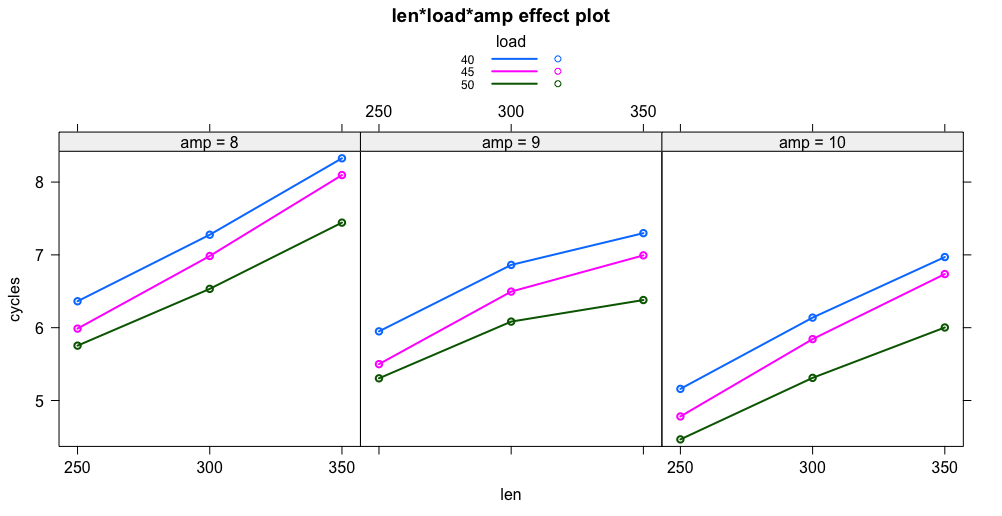
\includegraphics[width =\textwidth]{Rplot02.png}
      \end{center}
     \end{figure}    
     \textbf{Code:}
     \begin{center}
     \lstinputlisting[basicstyle = \small]{r9.txt}
     \end{center}
     \newpage

     \item[c.]Obtain estimates fo the level means of amp in the model that only contains main effects using emmeans().\\
     \solution Fitting the effects only model, and using the emmeans function we get, \\
     \textbf{Code:}
     \begin{center}
     \lstinputlisting[basicstyle = \small]{r10.txt}
     \end{center}
  \end{enumerate}
\end{exercise}





\end{document}





















